\providecommand{\main}{../../../..}
\documentclass[\main/dresen_thesis.tex]{subfiles}
\begin{document}
  \begin{figure}[tb]
    \centering
    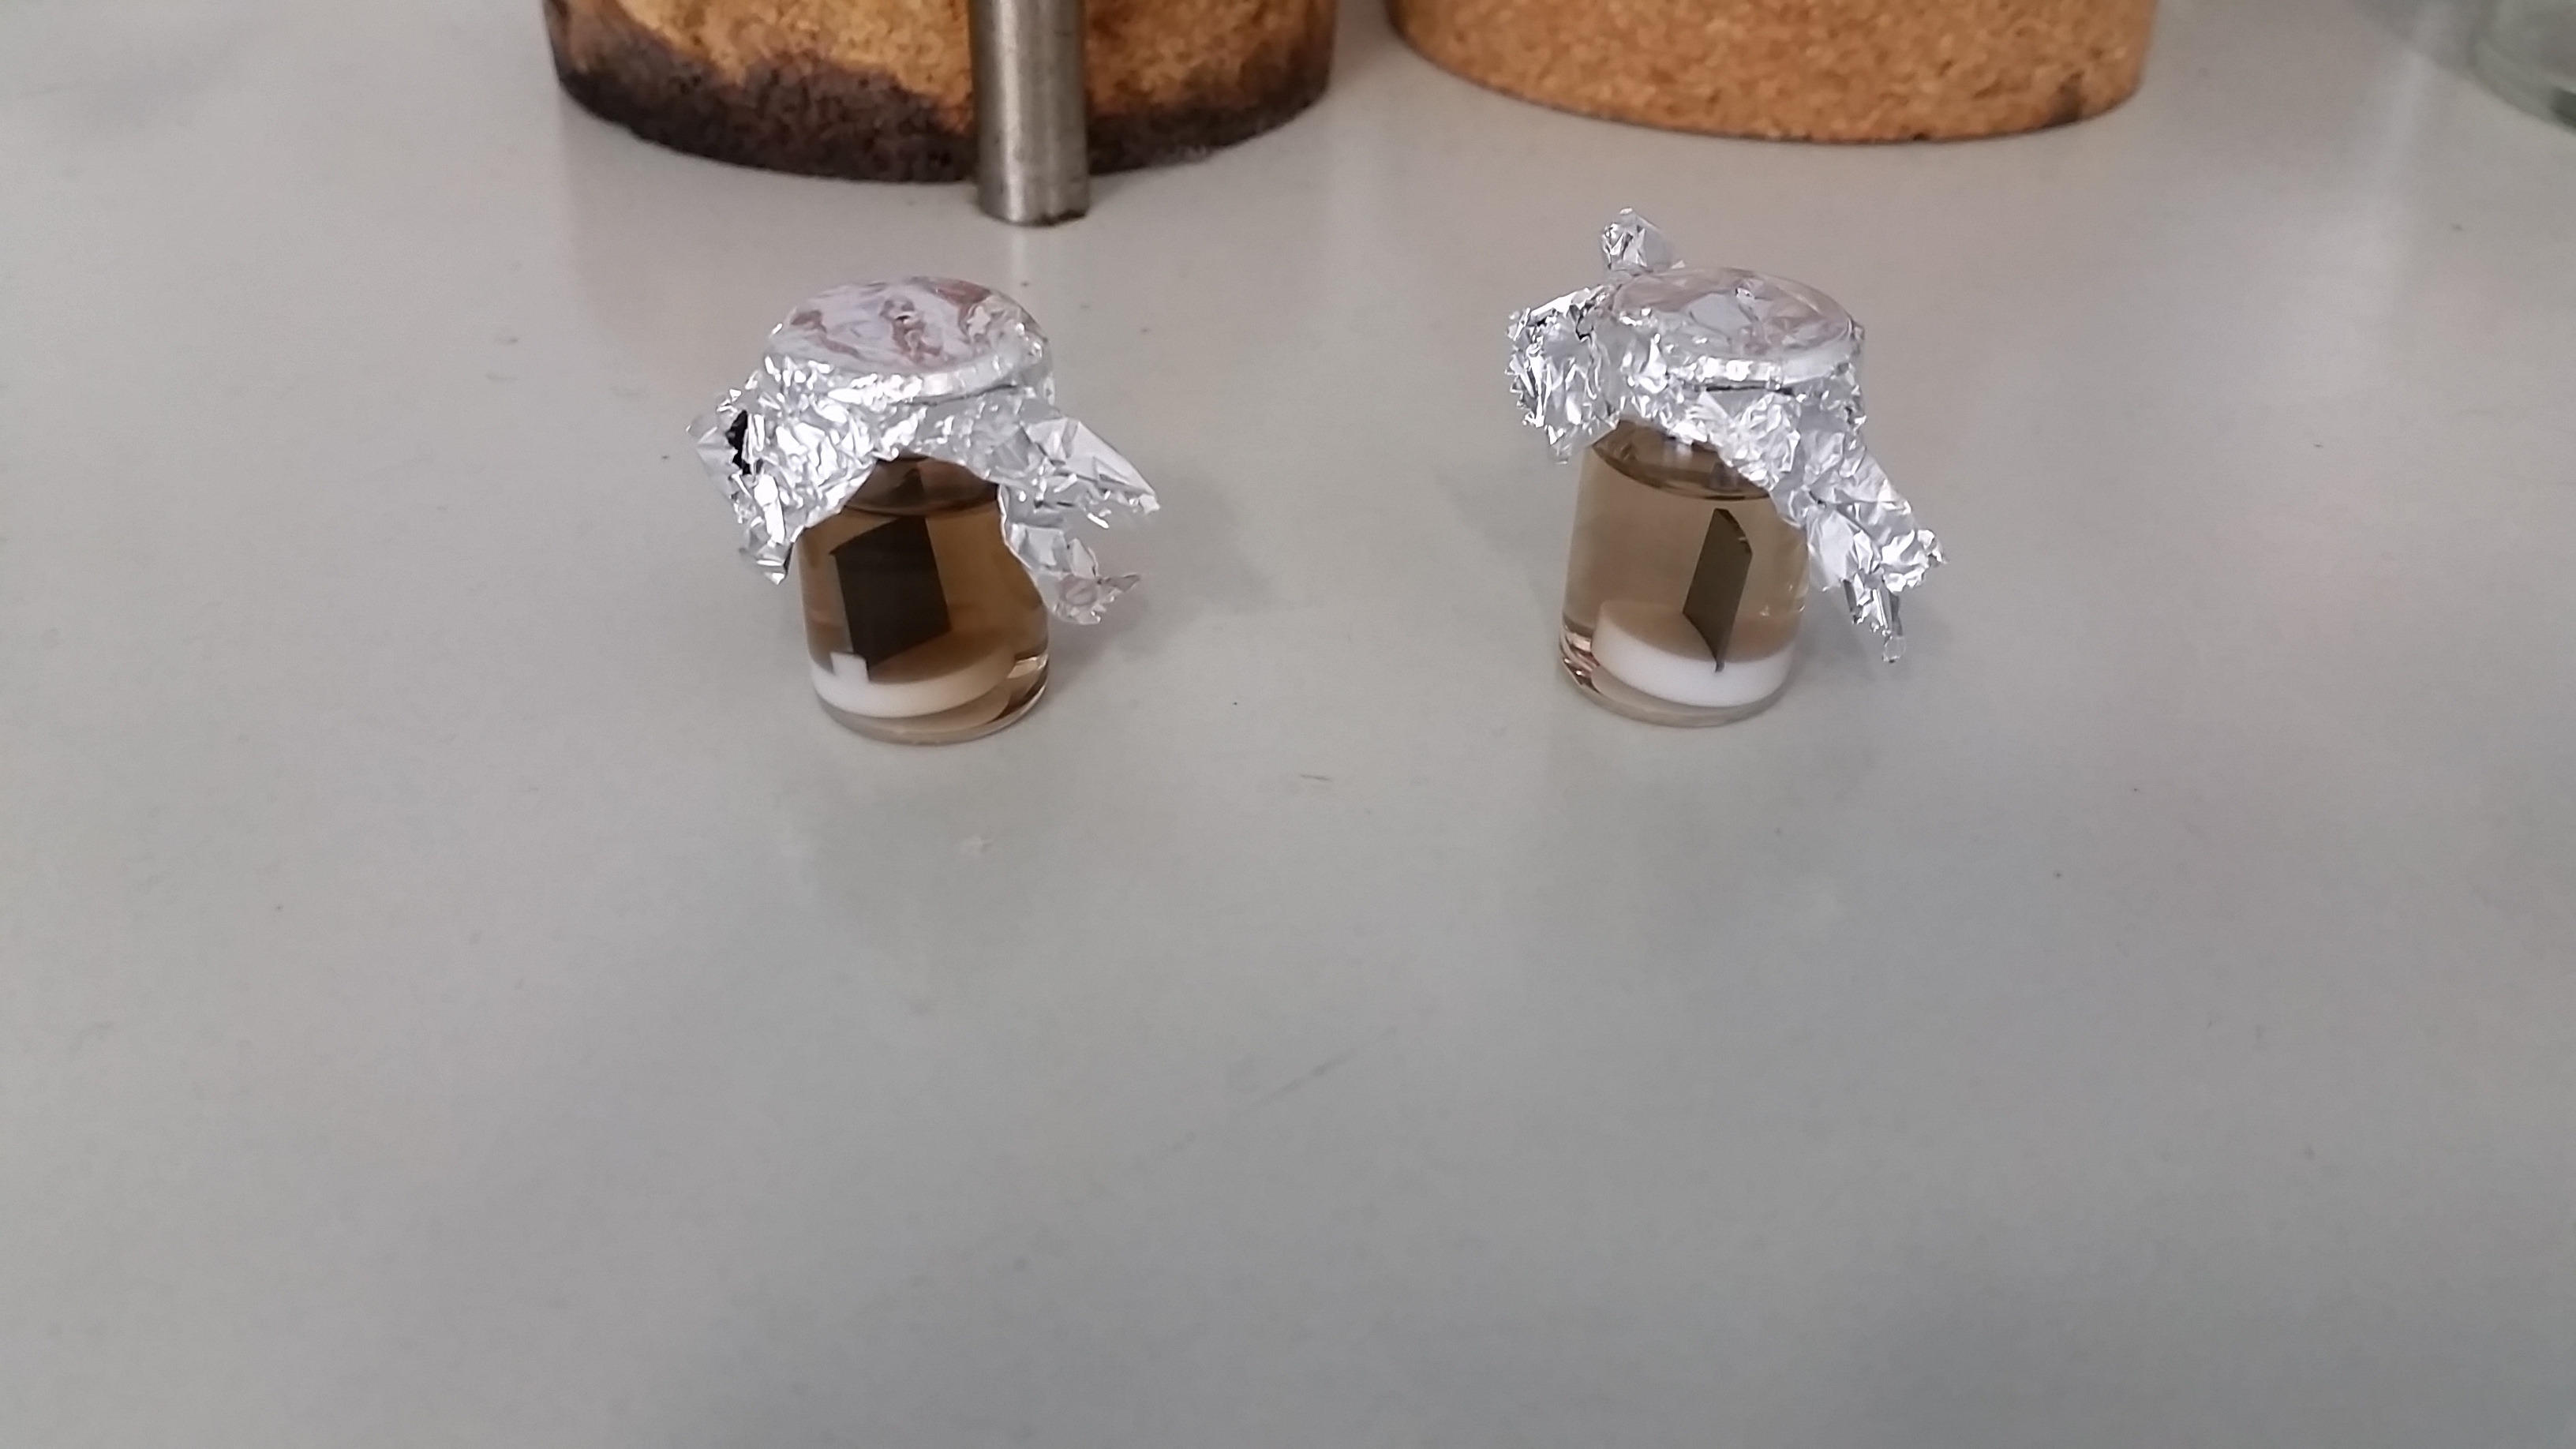
\includegraphics[width=0.79\textwidth]{colloidalCrystals_crystalPreparation}
    \caption{\label{fig:colloidalCrystals:preparation:image}Preparation of the colloidal crystals by the slow evaporation of a dispersion of nanoparticles on vertically fixated silicon substrates.}
  \end{figure}

  To achieve a long-ranged order three dimensional colloidal crystal, silicon substrates are vertically positioned in a slowly drying dispersion of the nanocubes Ol-Fe-C.
  For this purpose, the silicon substrates are first cleaned by washing them with ethyl acetate and isopropanol (HPLC grade) using a ultra-sonification bath for ten minutes each.
  The silicon substrate is fixed on a custom built Teflon platform and placed in a small beaker.
  Then $3 \unit{mL}$ of a toluene dispersion of nanocubes with a concentration of $c_m$ are filled in the beaker, which is tightly enclosed by aluminium foil.
  The used concentrations for the varied samples are tabulated in \reftab{tab:colloidalCrystals:preparation:conditions}.
  A single hole is punctuated in the center of the aluminium foil with a hypodermic needle of $0.9 \unit{mm}$ diameter to allow a slow evaporation of the dispersion.
  The beakers, shown in \reffig{fig:colloidalCrystals:preparation:image} are placed in an abandoned laboratory and allowed to evaporate without interference over a course of $1 - 2 \unit{weeks}$ until the solvent and the wafer surface has completely dried.

  \begin{table}[!htbp]
    \centering
    \caption{\label{tab:colloidalCrystals:preparation:conditions} Concentration of the Ol-Fe-C nanocubes in the dispersions used for the preparation of the colloidal crystals.}
    \begin{tabular}{ l | c }
      \textbf{Sample}               & $c_m \, /  \unit{mg \, mL^{-1}}$\\
      \hline
      \rule{0pt}{2ex} CC-Fe-0.25    & $0.25$\\
      \rule{0pt}{2ex} CC-Fe-0.37    & $0.37$\\
      \rule{0pt}{2ex} CC-Fe-0.50    & $0.50$\\
      \hline
    \end{tabular}
  \end{table}

\end{document}